\documentclass[12pt,a4paper]{article} 

\usepackage{fn2kursstyle}
\usepackage[russian]{babel}
\usepackage[T2A]{fontenc} 
\usepackage[utf8]{inputenc} 
\usepackage{geometry}
\usepackage{mathtools}
\usepackage{tikz}
\usepackage{pdfpages}
\usepackage{amsmath}
\usepackage[hidelinks]{hyperref}

\counterwithout{equation}{section}
\counterwithout{figure}{section}
\graphicspath{{pic/}}
\frenchspacing 

\newcommand{\picref}[1]{рис. \ref{#1}}
\newcommand{\half}{\frac{1}{2}}
\newcommand{\dhalf}{\dfrac{1}{2}}

\title{КУСОЧНО-ПАРАБОЛИЧЕСКИЙ МЕТОД НА ЛОКАЛЬНОМ ШАБЛОНЕ ДЛЯ ЗАДАЧ ГАЗОВОЙ ДИНАМИКИ}
\group{ФН2-62Б}
\author{А.\,И.~Токарев}
\supervisor{В.\,В.~Лукин}
\date{2022}

\begin{document}
    \maketitle
    \tableofcontents
    \pagebreak

    \section-{Введение}
    Одним из наиболее удачных вычислительных методов решения гиперболических уравнений является кусочно-параболический метод (с англ. Piecewise-Parabolic Method, PPM), разработанный для моделирования течения жидкостей и газов и применяемый в астрофизике. Он обладает порядком аппроксимации $ O(\tau^2 + h^3) $. Несмотря на великолепную точность, данный метод имеет ряд недостатков: концы парабол на разностных ячейках связываются путем реконструкции переменных на расширенном четырехточечном шаблоне, что повышает диссипацию в схеме. Кроме того, PPM дает достаточно точный результат на гладких решениях, а вот на разрывах происходят ощутимые осцилляции.

    Целью данной курсовой работы является анализ улучшенного метода PPM -- кусочно-параболического метода на локальном шаблоне (PPML). Его основное отличие заключается в том, что граничные точки парабол внутри разностых ячеек определяются с предыдущего временного слоя по методу характеристик, что позволяет точно описывать разрывные решения и избегать накопления лишней диссипации.
    
    В качестве анализа будет приведено сравнение точности методов PPM и PPML на примерах одномерных задач. Также проведем демонстрацию рассматриваемого метода на нескольких двумерных задач газовой динамики.

    \newpage
    
    \section{Постановка задачи}

    \subsection{Кусочно-параболический метод. PPM}
    Рассмотрим одномерную задачу. Пусть $\Omega_h$ -- множество узлов сетки, в общем случае неравномерной. Определим функцию $y(x)$ ее разностным аналогом $y_i, \, i = 1 \ldots n$ на этой сетке. Значения $y_i$ будем соотносить с центрами ячеек, а $ y_{ i + \half} = y_i^R $ и $ y_{i - \half} = y_i^L $ -- с концами. Строение разностной ячейки можно увидеть на \picref{fig:ppm_visual}

    \begin{figure}[h]
        \centering
        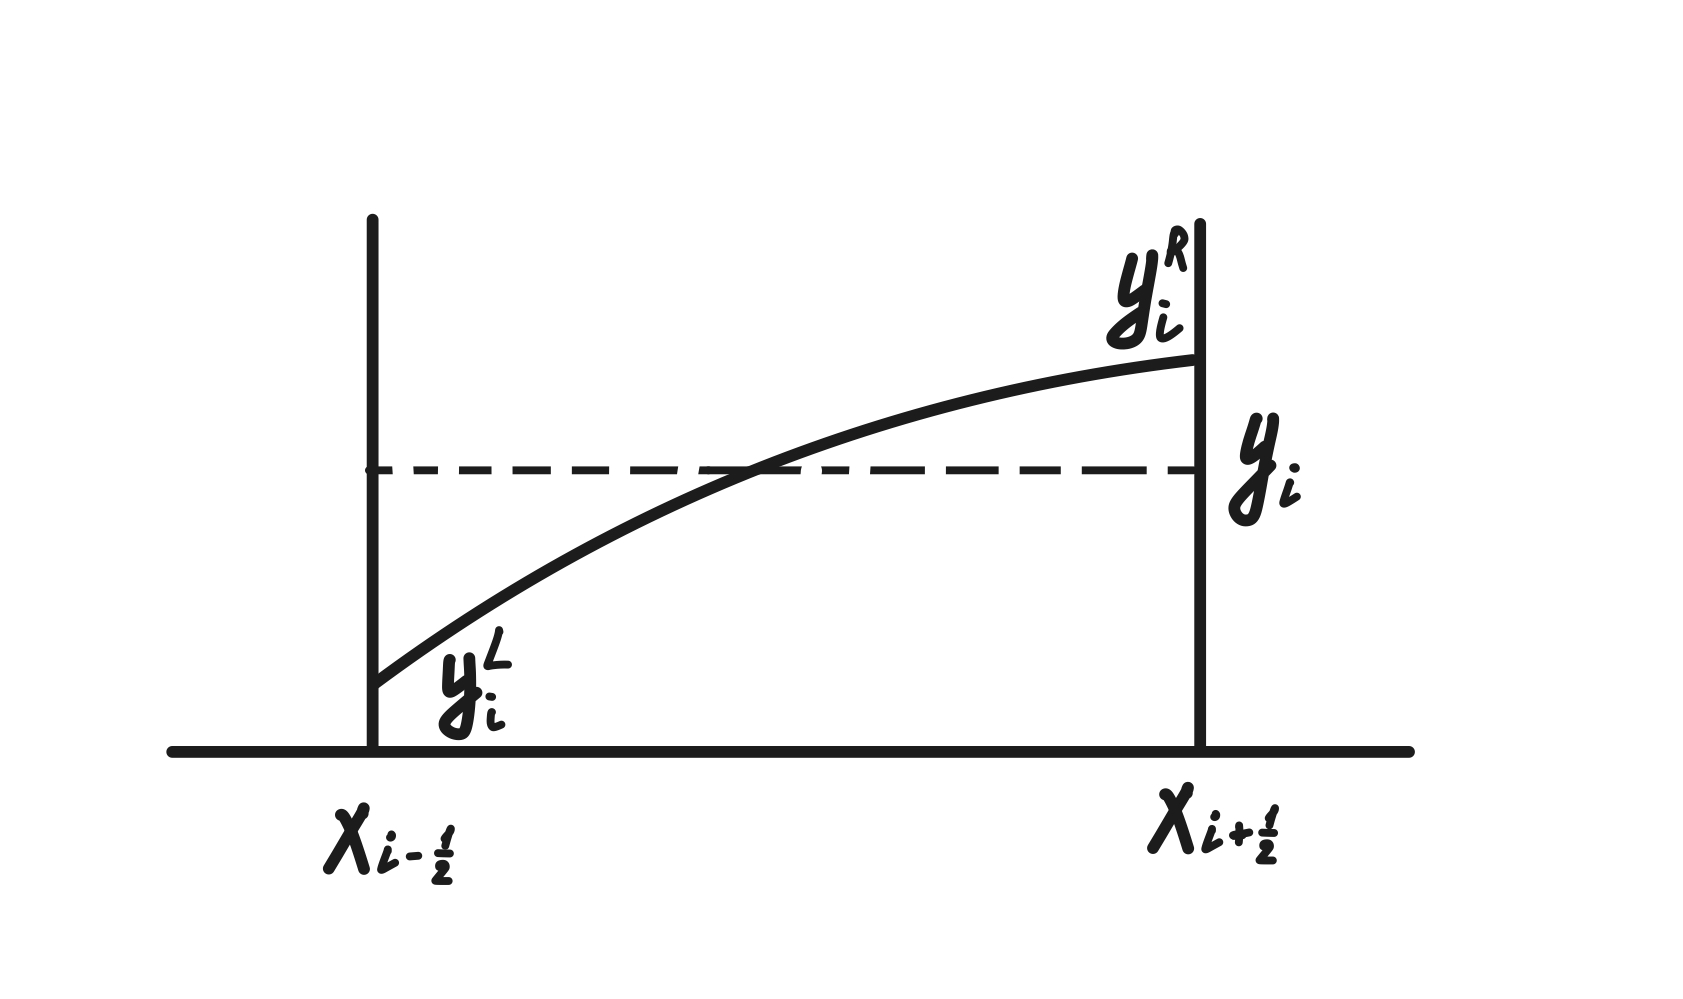
\includegraphics[width=0.5\textwidth]{ppm_visual.jpeg}
        \caption{Парабола внутри разностной ячейки}
        \label{fig:ppm_visual}
    \end{figure}

    Основная идея метода PPM заключается в следующем -- внутри отрезка $ [x_{i-\half}, x_{i+\half}] $ функцию $ y = y(x) $ можно аппроксимировать параболой:
    \begin{equation}
    \begin{split}
        \label{parabolic_eq}
        &y(x) = y_i^L + \xi(\Delta y_i + y_i^{(6)}(1 - \xi)), \quad \xi = (x - x_{i-\half})h^{-1}, \quad  \Delta y_i = y_i^R-y_i^L, \\
        &y_i^{(6)} = 6\Bigl[ y_i - \half(y_i^R + y_i^L)\Bigr], \quad x \in [x_{i-\half}, x_{i + \half}].
    \end{split}
    \end{equation}

    Выражение \eqref{parabolic_eq} является квадратурной формулой для соотнешния:
    \[
        y(x_i) = \dfrac{1}{h} \displaystyle \int_{x_{i-\half}}^{x_{i+\half}} y(\chi) d\chi.
    \]

   Значение функции $ y(x) $ на границах при условиях гладкости и отсутствия экстремумов принадлежит отрезкам:
   \begin{equation}
        \label{ppm_boundary}
        y_{i-\half} \in [y_{i-1}, y_i], \qquad y_{i+\half} \in [y_i, y_{i+1}], 
   \end{equation}
   \noindent далее производится монотонизация функции внутри каждой разностной ячеки, в результате чего меняются граничные значения, а приводит к появлению разрывов.

   Первым шагом ищем значение $y_{i+\half}$ интерполяционной процедурой четвертого порядка, в результате получаем значения:
   \[
        y_i^R = y_{i+1}^L = y_{i+\half} = \dhalf(y_i + y_{i+1}) - \dfrac{1}{6}(\delta y_{i+1} - \delta y_i),
   \] 
   \noindent где 
   \[
        \delta y_i = \dhalf(y_{i+1} + y_{i-1}).
   \]

    Чтобы обеспечить монотонность решения и выполнить условие \eqref{ppm_boundary}, значения $ \delta y_i $ нужно заменить на 
    \[
        \delta_m y_i = 
        \begin{cases}
            \min(|\delta y_i|,\, 2|y_i - y_{i-1}|,\, 2|y_{i+1} - y_i|)\cdot sign(\delta y_i), & (y_{i+1} - y_i)(y_i - y_{i-1}) > 0, \\
            0, \quad (y_{i+1} - y_i)(y_i - y_{i-1}) \leq 0.
        \end{cases}  
    \]

    После определения всех граничных точек переходим к следующему шагу. В областях немонотонного решения $ y(x) $ следует переопределять значения $ y_i^L,\, y_i^R $. При этом возможны два сценария:
    \begin{itemize}
        \item $ y_i $ является локальным экстремумом, тогда на всем отрезке $ [x_{i-\half}, x_{i+\half}] $ функция $ y(x) = \text{const} $, а значит:
        \begin{equation}
            \label{local_sup}
            y_i^L = y_i^R = y_i, \quad (y_{i+1} - y_i)(y_i - y_{i-1}) \leq 0;
        \end{equation}
                
        \item $ y_i $ лежит слишком близко к границе, а при условии $|\Delta y_i| < | y_i^{(6)} |$ парабола может иметь экстремум внутри разностной ячейки. В этом случае $ y_i^L $ и $ y_i^R $ должны быть выбраны так, чтобы сдвинуть его к границам:
        \begin{equation}
            \label{boundary_sup}
            \begin{split}
                y_i^L = 3y_i -2y_i^R, &\quad \Delta y_i \cdot y_i^{(6)} > (\Delta y_i)^2, \\
                y_i^R = 3y_i -2y_i^L, &\quad \Delta y_i \cdot y_i^{(6)} < -(\Delta y_i)^2.
            \end{split}  
        \end{equation}
    \end{itemize}

    После всех проделанных операция функцию $y(x)$ можно считать определенной на сетке $\Omega_h$. 
    
    Cреднее значение данной функции на отрезке $ [x_{i+\half}-\alpha, x_{i+\half}], (\alpha > 0) $ задается формулой:
    \begin{equation}
        \label{average_positive}
        \overline y_{i+\half}^L(\alpha) = \dfrac{1}{\alpha} \displaystyle \int_{x_{i+\half}-\alpha}^{x_{i+\half}} y(x) dx = y_i^R - \dfrac{\alpha}{2h}\Bigl[ \Delta y_i - \Bigl( 1 - \dfrac{2 \alpha}{3h} \Bigr)y_i^{(6)} \Bigr],
    \end{equation}
    \noindent а на отрезке $ [x_{i+\half}, x_{i+\half}+\alpha], (\alpha > 0)$:
    \begin{equation}
        \label{average_negative}
        \overline y_{i+\half}^R = \dfrac{1}{\alpha} \displaystyle \int_{x_{i+\half}}^{x_{i+\half}+\alpha} y(x) dx = y_{i+1}^L  + \dfrac{\alpha}{2h} \Bigl[\Delta y_{i+1} + \Bigl( 1 - \dfrac{2\alpha}{3h} \Bigr) y_{i+1}^{(6)} \Bigr].
    \end{equation}

    \subsection{Кусочно-параболический метод на локальном шаблоне. PPML}

    Интерполяционная процедура четвертого порядка, применяемая для переопределения граничных узлов, сглаживает разрывные решения $y(x)$. Чтобы обойти данное ограничение, можно определять $ y_i^L $ и $ y_i^R $ с помощью переноса значения на параболе с предыдущего шага по времени вдоль характеристики $ \frac{dx}{dt} = a $. Причем переопределять нужно лишь одну из границ. Для ясности  будем рассматривать $y_i^R = y_{i+\half}$. Для того, чтобы вычислить ее на следующем временном слое $ t_j + \tau = t_{j+1}$ (обязательное ограничение -- выполнение условия Куранта $ a \Delta t_j \leq \min_{0 \leq i \leq n}\Delta x_i $), необходимо двигаться от точки $ x_{i+\half} $ со значением $ y_{i+\half} $ вдоль характеристика до предыдущего момента времени $ t_j $:
    \begin{enumerate}
        \item $ a > 0 $, следовательно
        \begin{equation}
            \label{ppml_boundary}
            \begin{split}
                &y_{i+\half}(t_{j+1}) = y_i^R(t_{j+1}) = y_i^L(t_j) + \xi(\Delta y_i(t_j) + y_i^{(6)}(t_j)(1-\xi)), \\[0.7em]
                &\xi = \dfrac{x - x_{i-\half}}{h} = 1 -  \dfrac{a \tau}{h};
            \end{split}
        \end{equation}

        \item $ a < 0 $, следовательно
        \[
            \begin{split}
                &y_{i+\half}(t_{j+1}) = y_i^R(t_j) = y_i^R(t_j) + \xi(\Delta y_{i+1}(t_j) + y_{i+1}^{(6)}(t_j)(1-\xi)), \\[0.7em]
                &\xi = \dfrac{x - x_{i-\half}}{h} = 1 -  \dfrac{a \tau}{h}.
            \end{split}  
        \]
    \end{enumerate}

    Алгоритм \eqref{ppml_boundary} реализован на локальном шаблоне, то есть для получения граничных точкек при переходе на следующий временной слой не нужно использовать информацию с соседних ячеек. Нахождение среднего значения на отрезке \eqref{average_positive}, \eqref{average_negative} и смещение экстремума \eqref{local_sup}, \eqref{boundary_sup} производятся аналогично.

    \subsection{Потоки и усредненное значение на отрезке}

    При возникновении разрыва на границе двух смежных ячеек в точке $ x_{i+\half} $ возникает некоторое усредненное состояние $ y^\star(x_{i+\half}, t) $. Одномерное уравнение переноса имеет всего одну характеристику, поэтому его решение в момент времени $ t = t_{j+1} $ будет определяться:
    \begin{enumerate}
        \item При $ a > 0 $ усреднением по пространствунному интервалу $ [x_{i+\half}-a \tau, x_{i+\half}] $ со значением $ y^\star(x_{i+\half}, t_{j+1}) = \overline y_{i+\half}^L(a \tau) $;
        
        \item При $ a < 0 $ -- по интервалу $ [x_{i+\half} \tau, x_{i+\half}+a \tau] $ со значением $ y^\star(x_{i+\half}, t_{j+1}) = \overline y_{i+\half}^R(-a \tau) $.
    \end{enumerate}

    Поток на границе смежных ячеек в задаче Римана определяется по формуле:
    \begin{equation}
        \label{boundary_flow}
        \begin{split}
            &F_{i+\half} = \dfrac{1}{\tau} \displaystyle \int_{t_j}^{t_{j+1}} F(y^\star(x_{i+\half}, t))dt = a^+ y_{i+\half}^L + a^- y_{i+\half}^R, \\[0.5em]
            &a^+ = \max(0, a), \quad a^- = \min(a, 0).
        \end{split}
    \end{equation}

    \section{ Одномерное уравнение переноса }

    \begin{equation}
        \label{convection-diffusion}
      \dfrac{\partial q}{\partial t} + a \dfrac{\partial q}{\partial x} = 0.  
    \end{equation}

    Решением уравнения переноса является функция, сохраняющая свой профиль с течением времени, то есть $ y(x, t) = y_0(x-at) $, где $ u_0 $ -- начальный профиль. Это происходит по той причине, что профиль при сносе по характеристикам остается одинаковым. Если $\frac{dx}{dt} = a $ -- характеристика, то прямые $ x-at = b $ называют характеристическими. На каждой из таких прямых $ y = \text{const} $ и перемещается по ней с некоторой заданной скоростью $ a $. 

    Уравнение переноса – простейший пример, применяемый для проверки алгоритма на корректность. В задачах газодинамики оператор переноса является составной частью, поэтому любой численный метод для таких моделей обязан проходить проверку простейшим уравнением.

    Рассмотрим задачу Коши для линейного уравнения переноса \eqref{convection-diffusion} c различными начальными условиями $ y_0 \colon$
    \begin{gather*}
        y_0(x) = \dfrac{x - l_1}{l_2 - l_1} \text{ -- левый треугольник}, \\[1em]
        y_0(x) = \dfrac{l_2 - x}{l_2 - l_1} \text{ -- правый треугольник}, \\[1em]
        y_0(x) = 1 \text{ -- прямоугольник}, \\[1em]
        y_0(x) = \begin{cases}
            -\dfrac{2(x-l_1)}{3(l_{11}-l_1)} + 1, & x \in [l_1, l_{11}), \\[0.7em]
            \dfrac{1}{3}, & x \in [l_{11}, l_{22}], \\[0.7em]
            \dfrac{2(x-l_{2})}{3(l_2 - l_{22})} + 1, & x \in (l_{22}, l2], \quad \text{-- зуб},
        \end{cases}
    \end{gather*}
    \begin{gather*}
        y_0(x) = \begin{cases}
            -\dfrac{2(x-l_1)}{3(l_{12}-l_1)} + 1, & x \in [l_1, l_{12}), \\[0.7em]
            \dfrac{2(x-l_{2})}{3(l_2 - l_{12})} + 1, & x \in [l_{12}, l2], \quad \text{-- M},
        \end{cases}
    \end{gather*}
    \noindent где $ l = 520,\, l_1 = 10,\, l_2 = 30,\, l_{11} = \frac{50}{3},\, l_{22} = \frac{70}{3},\, l_{12} = 20,\, T = 400,\, h = 1,\, a = 1$.

    Численное решение будем сравнивать с точным, имеющим вид: 
    \[  y_0(x) = 
         \begin{cases}
            0, & x - at < l_1, \\
            u_0(x-at), & l_1 \leq x-at \leq l_2, \\
            0, x-at > l_2.
         \end{cases} 
    \]

    \section{Уравнение Брюггерса}

    \section-{Заключение}

\end{document}